
%(BEGIN_QUESTION)
% Copyright 2010, Tony R. Kuphaldt, released under the Creative Commons Attribution License (v 1.0)
% This means you may do almost anything with this work of mine, so long as you give me proper credit

Sketch connecting wires to allow this data acquisition unit (DAQ) to sense light on input channels \#3 and \#7, such that increasing light at each photocell generates an {\it increasing positive} signal voltage on each channel.  Note that all the analog input channels on this DAQ are single-ended, bipolar:

$$\includegraphics[width=15.5cm]{i04587x01.eps}$$

Recall that the electrical resistance of a photocell {\it decreases} with increasing light.

\vskip 20pt \vbox{\hrule \hbox{\strut \vrule{} {\bf Suggestions for Socratic discussion} \vrule} \hrule}

\begin{itemize}
\item{} A good problem-solving technique to apply in cases where we need to determine the direction of a change for a component's resistance in order to design a functioning circuit is to consider {\it limiting cases} for that component's resistance.  For example, instead of asking ourselves what would happen if the intensity of light {\it slightly}, we ask ourselves what would happen if light intensity changed {\it dramatically}.  Explain how this problem-solving technique applies to this particular system.
\item{} After you have sketched your circuit, evaluate the effects of various components failing either open or shorted, one at a time.
\end{itemize}

\underbar{file i04587}
%(END_QUESTION)





%(BEGIN_ANSWER)

If we need the signal voltage to increase with increasing light intensity, and we know a photocell's resistance decreases with increasing light intensity, we need the DAQ to sense voltage across the fixed resistor and not across the photocell.

$$\includegraphics[width=15.5cm]{i04587x02.eps}$$

%(END_ANSWER)





%(BEGIN_NOTES)


%INDEX% Pictorial circuit review (analog signal wiring to data acquisition unit)

%(END_NOTES)

